%%
%% This is file `yanputhesis-sample.tex',
%% generated with the docstrip utility.
%%
%% The original source files were:
%%
%% yanputhesis.dtx  (with options: `sample')
%% Copyright (C) 2022 by Shangkun Shen
%% 
%% It may be distributed and/or modified under the conditions of the LaTeX
%% Project Public License, either version 1.3b of this license or (at your
%% option) any later version. The latest version of this license is in
%%     https://www.latex-project.org/lppl.txt
%% and version 1.3b or later is part of all distributions of LaTeX version
%% 2005/12/01 or later.
%%=============================================================================%
%% 设置论文格式(学位、盲评、Adobe 字体)
%%-----------------------------------------------------------------------------%
%% 博士、正常版本、不使用 Adobe 字体
%% \documentclass[lang=chs, degree=phd, blindreview=false, adobe=false]{yanputhesis}
%% 博士、盲评版本、不使用 Adobe 字体
%% \documentclass[lang=chs, degree=phd, blindreview=true, adobe=false]{yanputhesis}
%% 博士、正常版本、强制使用 Windows 系统字体
%% \documentclass[lang=chs, degree=master, blindreview=false, winfonts=true]{yanputhesis}/
%% 硕士、正常版本、不使用 Adobe 字体
\documentclass[lang=chs, degree=master, blindreview=false, adobe=false]{yanputhesis}
%% 硕士、盲评版本、不使用 Adobe 字体
%% \documentclass[lang=chs, degree=master, blindreview=true, adobe=false]{yanputhesis}
%%=============================================================================%
%% 导言区:请自行添加额外宏包
%%-----------------------------------------------------------------------------%
\usepackage{blindtext}                                      % 生成无意义文本
\usepackage{metalogo}                                       % 软件标志
\usepackage[binary-units=true]{siunitx}                     % 物理量单位
\usepackage{amsmath}                                        % 基础数学库
%%=============================================================================%
%% 参考文献(也可以是独立文件)
%%-----------------------------------------------------------------------------%
\begin{filecontents}{reference.bib}
@inproceedings{chen2019vision,
	title={A vision based system for anomaly detection and classification in additive manufacturing},
	author={Chen, Wei Jie and Ho, Jee-Hou and Mustapha, Khameel Bayo and Chai, Tong-Yuen},
	booktitle={2019 IEEE conference on sustainable utilization and development in engineering and technologies (CSUDET)},
	pages={87--92},
	year={2019},
	organization={IEEE}
}

@inproceedings{vaikundam2016anomaly,
  title={Anomaly region detection and localization in metal surface inspection},
  author={Vaikundam, Sriram and Hung, Tzu-Yi and Chia, Liang Tien},
  booktitle={2016 IEEE International Conference on Image Processing (ICIP)},
  pages={759--763},
  year={2016},
  organization={IEEE}
}


\end{filecontents}
%%=============================================================================%
%% 基本信息录入
%%-----------------------------------------------------------------------------%
\title{面向工业图像的无监督 \\ 异常检测与定位研究}{          % 中英文标题
   The study of unsupervised anomaly detection and localization for industrial images
}                                                           % 请自行断行
\author{\blindreview{涂山川}}{\blindreview{Shanchuan Tu}}  % 姓名(添加盲评标记)
\date{2024年11月}{Nov 2024}                                  % 答辩日期
\school{光电与智能研究院}{School of Artificial Intelligence, OPtics and ElectroNics(IOPRN)}% 学院
\major{计算机科学与技术}{Computer Science and Technology}                     % 专业 博士请添加 Ph
\advisor{\blindreview{马单丹}}{\blindreview{Dandan Ma}}      % 导师(添加盲评标记)
\studentnumber{2022205223}                                  % 学号

%%=============================================================================%
%% 文档开始
%%-----------------------------------------------------------------------------%
\begin{document}
%%-----------------------------------------------------------------------------%
%% 总前言,包含封皮页、中英文标题、中英文摘要、目录
%%-----------------------------------------------------------------------------%
\frontmatter                                                % 前言部分
\maketitle                                                  % 封皮页及标题页
%%-----------------------------------------------------------------------------%
\makeCommitteePage{                                         % 学位论文评阅人
    \reviewers{\fullBlindReview{5}}                         % 和答辩委员会名单
    \committee{2023 年 x 月 y 日}{
        \defenseChair{赵钱孙}{教授}{西北工业大学}
        \committeeMember{周吴郑}{教授}{西北工业大学}
        \committeeMember{冯陈褚}{教授}{西北工业大学}
        \committeeMember{蒋沈韩}{教授}{西北工业大学}
        \committeeMember{朱秦尤}{教授}{西北工业大学}
        \committeeMember{何吕施}{教授}{西北工业大学}
        \committeeMember{孔曹严}{教授}{西北工业大学}
        \defenseSecretary{金魏陶}{教授}{西北工业大学}
    }
}
%%-----------------------------------------------------------------------------%
\begin{abstract}                                            % 中文摘要开始
    这是在西北工业大学本科毕业设计、硕博研究生毕业论文格式的要求下的一份 LaTeX
    文档类模板。使用者无需额外修改格式控制细节,直接在所发布的样例基础上,修改章
    节标题,撰写内容,即可完成毕业设计论文任务。            %
    \begin{keywords}                                        % 中文关键词开始
        学位论文 \sep 模板 \sep \LaTeX                      %
    \end{keywords}                                          % 中文关键词结束
\end{abstract}                                              % 中文摘要结束
%%-----------------------------------------------------------------------------%
\begin{engabstract}                                         % 英文摘要开始
    \noindent \blindtext                                    %
    \begin{engkeywords}                                     % 英文关键词开始
        thesis \ensep template \ensep \LaTeX                %
    \end{engkeywords}                                       % 英文关键词结束
\end{engabstract}                                           % 英文摘要结束
%%-----------------------------------------------------------------------------%
\tableofcontents                                            % 目录
\listoffigures                                              % 图目录(学校未做要求)
\listoftables                                               % 表目录(学校未做要求)
\printnomenclature                                          % 符号表(学校未做要求)
%%-----------------------------------------------------------------------------%
\mainmatter
\sDefault
\chapter{绪论}
\chaptermark{绪论}
\section{研究背景及意义}

从飞机机翼到芯片晶粒,工业产品在现代社会中无处不在,而产品质量控制在许多工业制造过程中是不可或缺的一步。随着技术的进步,基于视觉的自动异常检测在现代制造业中显著降低了人工和时间成本,并在智能制造系统中发挥着至关重要的作用。作为机器学习的一个重要分支,异常检测广泛应用于医学成像、自动驾驶和工业检查等领域,与我们的日常生活密切相关。异常检测,又称为离群点检测或异常数据检测,是一种利用无标注样本或正常样本构建检测模型的方法,旨在识别那些与其他数据显著不同或偏离预期模式的观测值或样本。

传统的工业图像异常检测与定位通常依赖专业仪器和经验丰富的技术人员进行手动干预,这不仅效率低下,且准确性难以保证。随着计算机视觉和图像处理技术的迅速发展,许多基于机器学习的算法被引入工业图像异常检测与定位,并取得了显著的成果,降低了成本,同时提高了效率和性能。传统方法中的监督学习算法通常需要大量带标签的数据来训练模型,但在实际工业生产中,获取大量异常图像数据非常困难,且为每个像素添加标签的成本高昂,这使得这些模型难以在真实场景中应用。因此,无监督异常检测(Unsupervised Anomaly Detection, UAD)方法引起了研究者们的关注。这些算法只需提供正常图像进行训练,而无需异常图像,因为在工业场景中,正常图像的数量通常远远超过异常图像,并且更容易获取。此外,无监督方法显著降低了标注成本,并避免了标签偏差可能带来的负面影响。

在基于视觉的工业智能背景下,工业图像异常检测与定位通过无监督学习方法,识别与正常图像不同的异常图像或局部异常区域。与仅判断图像是否异常不同,异常检测与定位的研究目标更为具体和实用。通过分割技术精确定位异常区域,帮助人们更好地理解异常的来源和性质,从而采取适当的措施进行处理和修复。工业图像异常检测不仅需识别异常样本,还需准确定位异常像素(即缺陷检测),但在这一过程中常常面临异常样本概率低和标注成本高等挑战。此外,工业图像的特点包括异常模式难以预知、异常可视性低、异常种类繁多以及图像背景复杂等,这使得精准定位异常变得更加困难。因此,如何有效检测工业图像中的异常并准确定位异常位置,对于实现产品质量控制和提升经济效益具有重要意义。

虽然基于传统特征工程的工业图像异常检测与定位技术已经取得了较为成熟的发展和应用,但此类方法由于需要手工设计缺陷的特征描述,当面对一些复杂无规则的图像缺陷时,难以准确地描述缺陷,且无法探测新型缺陷,这导致其应用发展受到阻碍。近年来,随着人工智能和计算机视觉的发展,深度学习广泛应用于工业图像异常检测于定位中。目前基于深度学习的无监督工业图像异常检测与定位方法主要分为基于图像重构的方法(Reconstruction based method)、基于嵌入的方法(Embedding based method)、基于正则化流的方法(Normalizing flow based method)和基于合成异常的方法(Synthesis based method)四类。基于图像重构的方法将输入图像编解码,以重构输入为目标训练神经网络,通过重构前后的图像差异来进行异常检测。该方法具有简单且速度较快的优点,该方法假设仅用正常数据训练的深度网络不能准确地重建异常区域,然而这种假设并不总是成立,有时一个网络也可以很好地重构异常输入,导致误检测。基于嵌入的方法通常使用ImageNet预训练的卷积神经网络来提取广义的正常特征,然后采用多元高斯分布、内存库等统计算法嵌入正态特征分布,最终通过将输入特征与学习分布或记忆特征进行比较来检测异常。然而,工业图像的特征分布通常与ImageNet不同,直接使用这些有偏差的特性可能会导致不匹配的问题,以及在正/负样本分布不均的情况下,此类方法难以捕获数据中复杂特征和模式。此外,统计算法总是存在高计算复杂度或高内存消耗的问题,这也限制了基于嵌入的方法的应用。基于正则化流的方法利用可逆变换直接构造正态分布,异常特征会落在分布的边缘从而实现异常检测。此类方法假设提取的正态数据的特征服从一定的分布,如多元高斯分布,并使用正态数据集来估计参数,然后通过推理将离群值数据识别为异常数据。由于实际数据并不一定符合高斯分布的假设,于是借用正则化流的思想,将任意分布投影到高斯分布来实现近似。然而通常情况下此类方法在推理构建分布时需要消耗大量时间,难以保证实时性的图像异常检测的任务需求。而基于合成异常的异常检测方法通过在训练过程中生成人工模拟的异常样本,并将其作为数据增强的一种形式,其目的是为了引入异常区分信息,减轻将所有正常样本映射到同一点所可能导致的过拟合问题。然而,此类方法对于一些图像前景和背景无法很好区分的数据集存在异常模拟效率低等问题,其面临着模拟异常方向性和可控性的挑战。

基于深度学习的方法在工业图像异常检测与定位中发挥着重要作用。然而,尽管一些现有方法取得了一定成效,但仍面临诸多挑战。首先,从数据分布的角度出发,由于异常样本稀缺,异常样本与正常样本的数量通常存在严重的类别不平衡问题,现有方法大多通过提取正常样本特征,并结合非参数分布估计方法来表征相应的分布,却忽略了局部特征与全局特征之间的关系,导致现有的异常检测模型识别异常样本的能力和泛化性能较弱。其次,从异常形式的角度出发,由于工业图像中不同异常的大小变化不可预测以及异常类型的多样性,导致现有的无监督异常检测与定位算法仍无法完全具备检测出各种样式的异常的能力,其本质是没有提取出有区分性的关键特征或者所提取的特征中存在一定的冗余。最后,从异常差异的角度出发,现有方法充分关注了仅使用正常样本进行模型训练,致力于高效地探索正常样本的通用模式,而对特定异常的关注较少。在真实的工业场景中,往往同一生产线上产品的类内差异较小,其产生的差异性影响导致异常的定位显著性不明显的问题,且异常缺陷以各种形式出现,仅使用正常样本而不与非正常样本进行比较并不足以让模型了解什么是正常模式。因此,基于以上研究发现,本文将对面向工业图像的无监督异常检测与定位算法进行研究。

《中国制造2025》行动纲领白皮书\cite{李培根2016中国制造}提出,“建设制造强国任务艰巨而紧迫,需要加速推进信息化与工业化的深度融合,推进生产过程的智能化”。国务院在2017年印发了《新一代人工智能发展规划》,特别表示要在大数据智能理论领域重点突破无监督学习等难点问题,形成从大数据到知识、从知识到决策的学习能力\cite{国防2017国务院印发《新一代人工智能发展规划》}。因此,本研究基于深度学习和数据挖掘理论,面向无监督学习、图像处理和分析等具体任务,积极迎合国家发展战略规划,不仅将有效促进异常检测与定位理论发展,还将在多行业的医学影像、环境监测、安防监控等众多实际应用中发挥积极作用,具有重要的研究意义。

\section{国内外研究现状}

近年来,国内外在利用传统机器学习方法进行图像异常检测与定位方面已有诸多应用。随着深度学习技术的发展,越来越多的方法开始尝试结合神经网络以实现图像异常检测与定位。总体来看,现有的图像异常检测与定位方法可以根据模型构建阶段是否涉及神经网络,分为传统方法和基于深度学习的方法两大类别。

\subsection{基于传统方法的图像异常检测与定位}

传统方法的图像异常检测与定位一般会学习一个模型来描述正常图像,然后在检测阶段根据待检测图像与现有模型之间的匹配程度来进行异常检测。基于传统方法的图像异常检测与定位可根据异常检测原理分为以下类别:基于模版匹配、基于统计模型、基于稀疏编码重构和基于分类面构建的图像异常检测与定位方法。

\subsubsection{基于模版匹配的图像异常检测与定位}
在图像异常检测任务中,最理想的情况是所有的正常图像都高度相似,且异常图像与正常图像之间只会在小部分区域出现区别。此时,模板匹配是非常有效的一类异常检测方法。得到待检测图像与模板图像之间的对应关系之后,比较两者的差异可实现异常检测。Chen等人\cite{chen2019vision}提取待测图像和模板图像的 Hu 矩作为特征对三维打印零件进行异常与否的分类,Vaikundam 等人\cite{vaikundam2016anomaly}先提取了图像的 SIFT 特征,利用聚类算法进行描述符筛选之后,找到最为匹配的正常图像作为模板来进行异常区域的定位。Herwig等人\cite{herwig2013adaptive}则是通过中值滤波创建模板图像来检测钢材表面的异常区域,考虑到空域模板匹配方法容易受到诸如光照变化和正常图像间微小差异的影响,Tsai等人\cite{tsai2018defect}将模板匹配过程迁移到了频域,通过比较待检图像和模板图像经傅里叶变换后的频域分量来定位印制电路板上细微的缺陷。模板匹配的方法一般适用于图像采集环境稳定且可控的场景,然而在更多的情况下,即便是正常图像之间都会存在着较多的差异,难以通过模板匹配实现异常检测与定位。

\subsubsection{基于统计模型的图像异常检测与定位}
此类方法通常利用统计模型来描述正常图像中像素值或者特征向量的分布,而对于一些远离该分布的图像区域则认为存在异常。其中较为常见的方式是利用高斯模型进行描述,比如Reed等人\cite{reed1990adaptive}提出的RX(Reed-xiao)算法就利用高斯分布函数来描述高光谱图像中像素点内信息的分布情况\cite{du2010random}。然而一个高斯分布模型很难描述更为复杂多变的场景,为了进一步地提升建模效果,Veracini 等人\cite{veracini2009fully}通过高斯混合模型对高光谱图像的背景像素进行描述,并通过期望最大化算法来自适应地确定高斯混合模型中子分布模型的数量。Zhang等人\cite{zhang2018automatic}则是利用马尔科夫随机场提升了高斯混合模型的鲁棒性,在钢板表面获得了较好的异常定位效果。上述方法大多仅对像素点内的信息进行了建模而忽略了区域信息,且此类方法大多都预先对图像数据的分布做了假设,这在一定程度上降低了该方法的通用性。

\subsubsection{基于稀疏编码重构的图像异常检测与定位}
此类方法通常借助稀疏编码的方式对图像进行重构,并在此过程中学习一个字典来表示正常图像,然后在测试阶段从重构差异和稀疏度等角度进行异常检测与定位。Liang等人\cite{liang2016touch}依据编码向量的稀疏度来进行触摸屏表面的异常检测。Boracchi等人\cite{carrera2016defect}在稀疏度的基础上联合考虑重构误差来进行纳米材料表面的异常检测。Carrera等人\cite{carrera2016scale}则在传统的稀疏编码中结合了多尺度的策略,对于原始图像进行不同比例的缩放并分别构建字典,通过这种方式来提升对不同大小异常区域的检测性能。Chen等人\cite{chen2011sparse}在考虑稀疏度和重构精度的同时,对图像局部区域的平滑性同样进行了约束以得到更高质量的字典和重构过程。基于稀疏编码的方法不需要预先对数据的分布做假设,仅使用足够的样本就能很好地学习到正常图像的表示方法,这使得稀疏编码比之前的方法拥有更为广泛的应用场景,然而稀疏编码需要较多的空间来保存字典,导致此类方法会占用较多的存储空间,也会降低算法的运行速度。

\subsubsection{基于分类面构建的图像异常检测与定位}
此类方法希望在正常图像分布区域外构建一个足够紧致的分类面以区分正常样本和潜在的异常样本。较为经典的两类方法为单类支持向量机(One-class support vector machines, OC-SVM)\cite{scholkopf1999support, amraee2018abnormal}的方法和支持向量描述数据(Support vector data description, SVDD)\cite{tax2004support}方法。OC-SVM通过在高维空间创建超平面来分割正常样本和潜在异常样本,而SVDD则通过创建超球面来包裹绝大部分正常样本来实现异常检测与定位。Amraee等人\cite{amraee2018abnormal}提取图像中每一个区域的 HOG 和局部二值模式(Local Binary Pattern, LBP)等特征,然后借助 OC-SVM 对图像中每一个区域进行异常与否的分析。Azami等人\cite{el2015combining}对脑部核磁共振图像提取多种特征之后,结合OC-SVM进行异常区域的检测。Zhang等人\cite{zhang2010anomaly}和Gurram等人\cite{gurram2011hyperspectral}都将SVDD引入到了高光谱图像的异常检测任务中,Liu等人\cite{liu2010fast}提出了加速SVDD以实现液晶屏表面细微缺陷的实时检测。OC-SVM 模型简单而且有较为成熟的优化算法,不过随着样本维度的上升,其效果会受到显著的影响,且在面对定量异常时,大多需要通过区域划分的方式进行定位,这反而降低了算法的处理效率。

\subsection{基于深度学习的图像异常检测与定位}

近年来,深度学习在计算机视觉中的各个领域内都得到了长足的发展。相比于传统的方法,深度学习由于其无需人工设计特征,算法通用性更高等优点,已经被广泛引入到了图像异常检测与定位任务当中。现有的方法大致可以分为以下四类:基于图像重构的方法、基于嵌入的方法、基于正则化流和基于合成异常的方法。

\subsubsection{基于图像重构的图像异常检测与定位}
研究人员使用自动编码器、变分自动编码器或生成对抗网络在正常数据上训练图像重建模型,并以重构输入为目标训练神经网络,以此来学习正常图像的分布模式,然后在检测阶段通过分析重构前后图像之间的差异来进行异常检测。Mei等人\cite{mei2018unsupervised}利用降噪自编码器来进行纹理图像的异常区域定位,将样本切分成一系列小的图像片并分别进行重构,还表明结合多尺度的策略\cite{lin2017feature}在多个不同尺度下对图像进行重构可以有效地提升异常的定位精度基于嵌入的图像异常检测。Gong等人\cite{gong2019memorizing}提出的记忆强化自编码器,即在自编码器的基础上通过引入一个记忆模块,存储最具有代表性的特征向量以提升图像重构的稳定度。Schlegl等人\cite{schlegl2017unsupervised}提出的基于GAN的异常检测模型从某个随机变量开始,计算该变量生成的图像和待测图像之间的差异,通过梯度下降的方式迭代优化该随机变量,使得生成的图像逐渐接近待测图像。上述几种方法在检测阶段的优化过程较为烦琐且耗时,而Yang等人\cite{yang2019multiscale}在隐变量层增加了基于聚类损失的正则项来避免重构出异常区域,在纹理图像上的效果较好,但缺乏理论上的保证。

\subsubsection{基于嵌入的图像异常检测与定位}
基于嵌入的方法通常使用ImageNet\cite{deng2009imagenet}预训练的卷积神经网络来提取广义的正常特征,然后采用多元高斯分布\cite{defard2021padim}、内存库\cite{roth2022towards, gong2019memorizing, hou2021divide, yang2020improving}等统计算法嵌入正态特征分布,最后通过将输入特征与学习分布或记忆特征进行比较来检测与定位异常。例如,FYD\cite{zheng2022focus}设计了一个两级粗到细的特征对齐网络,学习正态图像的鲁棒特征分布;SPADE\cite{cohen2005sub}将KNN异常检测方法扩展到像素级,通过测试图像与正常图像之间的像素级对应来定位图像中的异常,而PaDiM\cite{defard2021padim}将提取的多元高斯分布嵌入异常斑块特征。PatchCore\cite{roth2022towards}使用最大代表性的内存库,在测试中采用马氏距离或最大特征距离对输入特征进行评分。然而工业图像的分布通常与ImageNet不同,直接使用这些有偏差的特性可能会导致不匹配的问题,这限制了在不可预见的情况下的泛化性能。此外,中间过程所包含的统计算法总是存在高计算复杂度或高内存消耗的问题。

\subsubsection{基于正则化流的图像异常检测与定位}
正则化流\cite{rezende2015variational}是一种具有双射映射和可追踪雅可比行列式的可逆神经网络,因为其可逆性有助于防止模态崩溃,此类方法通常用来估计正常数据的和潜在的异常数据分配的概率密度\cite{serra2019input}。最初,NICE\cite{dinh2014nice}提出了具有酉雅可比行列式的加性耦合层,而RealNVP\cite{dinh2016density}进一步提出了仿射耦合层,可以生成非体积保持映射。然而,Kirichenko等人\cite{kirichenko2020normalizing}揭示了在原始RGB图像上训练的流模型通常分配异常的概率可能性高于正常数据,因此可以通过将正则化流模型应用于高维度特征而不是原始图像。例如,DifferNet\cite{rudolph2021same}实现了正则化流模型流用于特征提取功能,并为了处理缺陷大小的变化,DifferNet将图像转换为3个尺度并通过相同的特征提取器提取多尺度特征图。而CFlow-AD\cite{gudovskiy2022cflow}利用不同效率水平和不同感受野的特征图构建其多尺度特征金字塔。然而,该方法忽略了空间上下文信息,导致全局感知丢失和局部感知脱节,最终导致在图像异常检测任务上性能表现不佳。最近,PyramidFlow\cite{lei2023pyramidflow}通过基于潜在的基于模板的缺陷对比定位范式来减少类内的方差,进而改进异常定位性能。

\subsubsection{基于合成异常的图像异常检测与定位}
为了使模型明确学习正常和异常样本之间的潜在差异,一些研究\cite{zavrtanik2021draem, li2021cutpaste, song2021anoseg}尝试在训练过程中生成人工模拟的异常样本,其目的是引入异常区分信息,并减轻将所有正常样本映射到同一点所可能导致的过拟合问题。例如,CutPaste\cite{li2021cutpaste}和AnoSeg\cite{song2021anoseg}采用类似“复制和粘贴”的增强方法,通过剪切正常区域并将其粘贴到随机位置,以模拟异常样本;NSA\cite{schluter2022natural}使用泊松图像编辑技术,将不同大小的图像块无缝融合,从而合成一系列更接近自然子图像不规则性的异常;而DRAEM\cite{zavrtanik2021draem}通过使用柏林噪声创建二值掩码,并在正常图像中填充外部纹理来合成异常。最近,已有一些方法在特征空间中进行合成异常。例如,DSR\cite{zavrtanik2022dsr}在量化特征空间中进行采样,并通过对代码本特征向量的相似性比较来合成弱缺陷异常;而SimpleNet\cite{liu2023simplenet}和UniAD\cite{you2022unified}通过在正常特征上添加高斯噪声来合成异常。然而,尽管现有方法在异常合成上能够提供细致的异常纹理,但仅单方面考虑了结构异常或者纹理异常,缺乏多样性,对于某些数据集图像中的目标前景和背景无法很好地区分,存在异常合成效率较低的问题。

\section{本文主要工作}
工业图像因为复杂多样的异常形式(例如异常尺寸不固定、异常类别繁多)、纹理多样性(例如结构纹理、重复纹理等)以及异常存在的低概率性等问题导致对其进行异常检测与定位更具挑战性。本研究以工业图像为研究对象,面向数据挖掘任务场景,围绕工业图像的异常检测和定位整体框架展开研究,并分别从数据分布、异常形式和异常差异三个方面对工业图像异常检测与定位算法展开研究。

\autoref{fig:Main Work}展示了本文研究工作的主要概览。整体上,本文的主要工作包含以下三个部分:

从异常检测与定位的数据分布出发,针对异常样本与正常样本分布不均匀导致模型的泛化能力较低,以及现有方法采用非参数分布的估计方法导致忽略了局部特征与全局特征之间的关系。本文提出了基于记忆正则化流的工业图像异常检测与定位算法(MemFlow)。所提出的算法结合二维正则化流与记忆增强模块,对全局特征和局部特征进行有效建模,并构建正常样本特征分布模式的记忆项和读取记忆项的寻址操作库,提高模型泛化能力和推理速度,并通过端到端的方式缓解目标域与源域特征分布不一致的问题。

从异常检测与定位的异常形式出发,针对工业图像中存在的多种异常形式,导致模型难以提取具有区分性的关键特征,以及对于存在细微缺陷的图像中模型无法提供有效区分边界异常的特征表示空间的问题,本文提出基于多尺度特征流的工业图像异常检测与定位算法(MultiFlow)。所提出的算法将嵌入的预训练卷积神经网络与多尺度流模型结合,利用低层次阶段的激活输出构建多尺度特征金字塔,并设计了非对称平行流与融合流的组合以进行特征的多尺度交换感知,以提取关键特征,最后采用不同的聚合策略增强对细微缺陷的鲁棒性与敏感性。

从异常检测与定位的异常差异出发,针对同一生产线上产品的类内差异较小导致在处理图像时难以区分,使得模型不足以容纳正常样本类内差异的问题,本文提出基于差异共和性的工业图像异常检测与定位算法(DiffSeg)。所提出的算法利用人工合成的模拟异常图像在训练阶段使模型有意识地区分正常与异常,模型在获得更鲁棒的决策边界的同时辅助模型更有方向性的方式进行学习,然后结合空间注意力模块加强对异常区域的最佳差异信息的猜测,以此提升异常检测与定位性能。

\begin{figure}[htb]
	\centering
	\includegraphics[width=1\linewidth]{figs/本文工作.png}
	\caption{本文主要工作概览图}
	\label{fig:Main Work}
\end{figure}

\section{本文组织工作}

本文主要由六个章节组成,每个章节的主要内容如下:

第一章:绪论。该章节首先介绍了本文研究的工业图像异常检测与定位问题以及研究背景与意义。然后介绍了国内外对该问题的研究现状,并将现有工作分为基于传统方法和基于深度学习两类方法分别进行介绍。接着介绍了本文的主要工作。最后对本文的组织结构与行文安排进行了说明。

第二章:相关技术。该章节首先介绍了异常检测与工业图像异常检测与定位的定义与检测定位流程。然后概述了图像异常检测与定位技术所涉及到的相关技术,包括自编码器、卷积神经网络、残差网络及注意力机制。最后对本文所采用的数据集与检测与定位评价指标进行了说明。

第三章:基于记忆正则化流的工业图像异常检测与定位算法。该章节首先对研究的问题进行概述。然后针对该问题详细介绍了所提出的基于记忆正则化流的工业图像异常检测与定位算法,包括整体架构、特征提取、记忆正则化流、记忆增强以及异常检测与定位过程。最后在基准数据集上开展了对比实验,并对实验结果进行了详细分析。

第四章:基于多尺度特征流的工业图像异常检测与定位算法。该章节首先对研究的问题进行概述。然后针对该问题详细介绍了所提出的基于多尺度特征的工业图像异常检测与定位算法,包括整体架构、多尺度特征提取、平行流与融合流、聚合策略以及异常检测与定位过程。最后在基准数据集上开展了对比实验,并对实验结果进行了详细分析。

第五章:基于差异共和性的工业图像异常检测与定位算法。该章节首先对研究的问题进行概述。然后针对该问题详细介绍了所提出的基于差异共和性的工业图像异常检测与定位算法,包括整体架构、异常模拟策略、差分记忆、特征融合与空间注意机制及异常检测与定位过程。最后在基准数据集上开展了对比实验,并对实验结果进行了详细分析。

第六章:总结与展望。该章节总结了本文的主要研究内容,并展望了未来工作的研究方向。

\chapter{相关工作}

\section{引言}

异常检测作为当下的热门研究方向,与许多学科的研究存在交叉,此外,挖掘异常值有助于及时决策,规避潜在风险。而工业图像中的异常往往具有未知性、不规则性与稀缺性,例如颜色的变化、表面缺陷大小未知、裂痕、破损等,使得工业图像精准的异常检测与定位更具有挑战性。本章首先阐述了异常检测与工业图像的异常检测与定位所设计到的相关定义,包括异常的定义及类型等。其次,对目前异常检测与定位领域常用的深度学习算法框架,包括自编码器、卷积神经网络等算法框架进行了介绍。最后,介绍了用于评价图像异常检测与定位的性能指标与基准数据集。

\section{异常检测}
\subsection{异常的定义及类型}

异常是指偏离预期模式范围的项目或事件,也通常被称为“离群值”或者“偏差”。Hawkins等人\cite{hawkins1980identification}对异常的定义得到了学术界的普遍认可,他们提到,“An outlier is an observation which deviates so much from the other observations as to arouse suspicions that it was generated by a different mechanism”。即异常值是由不同机制产生的与其他观察不同的现象。异常主要有两个特点:1)相对于正常样本,异常样本的数量占比较低;2)异常样本与正常样本存在明显的差别。一般情况下,异常主要分为简单异常和复杂异常。其中,简单异常也称为“点异常”。简单异常是指数据中出现一些与正常样本数据分布有较大偏差的数据点,如\autoref{fig:Three abnormal types}(a)所示的红色数据点,由于其偏离了正常样本点的分布区域而被视为异常点。而复杂异常又可以分为上下文异常和集群异常。其中,上下文异常指数据点虽然属于正常范围,但在特定场景中与周围数据对比显得与众不同,不符合上下文的规律,如\autoref{fig:Three abnormal types}(b)所示,$t_2$ 点的气温虽然在正常范围内,但通过联系前后两个月的气温并结合规律,就能发现该点应当属于异常数据。而集群异常,又称为模式异常,是指在一系列观测结果集合中,单个数据观测时都属于正常类型数据,但是多个数据聚合而成的结果与正常数据存在差异的异常类型,如\autoref{fig:Three abnormal types}(c)所示,箭头所指的区域内单独看每个点的值都属于正常范围,但这些点聚合在一起就形成了与正常模式完全不同的结构。

\begin{figure}[H]
	\centering
	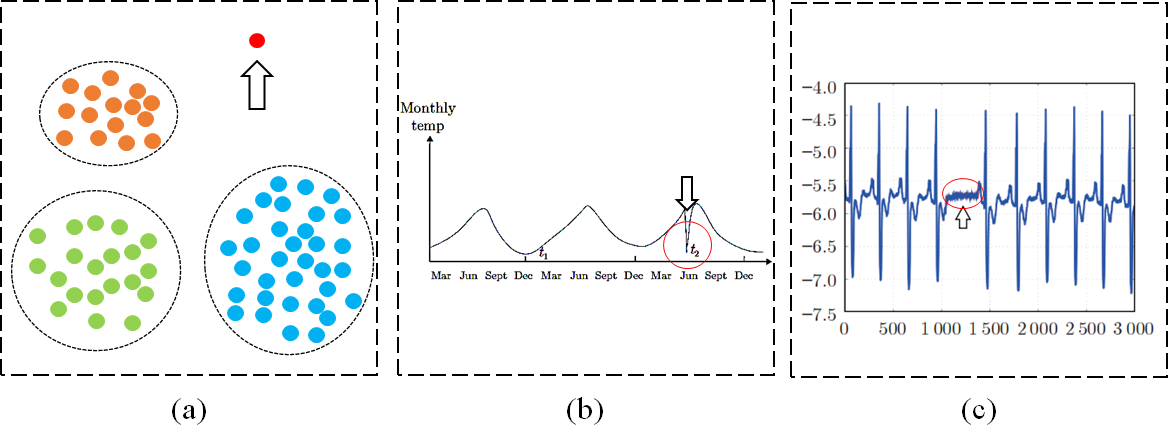
\includegraphics[width=1\linewidth]{figs/三种异常类型.png}
	\caption{不同异常类型示例}
	\label{fig:Three abnormal types}
\end{figure}


\subsection{异常检测的定义}

异常检测(Anomaly Detection, AD)是指在数据中识别与预期行为模式不符的样本或挖掘非逻辑数据的过程\cite{hodge2004survey}。异常数据可能蕴含重要信息,例如,在金融领域\cite{abd2021deep},银行等机构使用异常检测技术来监控客户的交易活动,以识别其中可能存在的欺诈行为;而在网络监控领域\cite{simmross2011anomaly},网络流量的异常可能意味着潜在的安全威胁或入侵行为。异常检测涵盖了多种下游任务,包括视觉异常检测和网络流量异常检测等。其中,视觉异常检测在工业外观缺陷检测\cite{jian2017automatic}、安防监控\cite{sabokrou2018deep}、医学图像分析\cite{roth2015anatomy, schlegl2017unsupervised}和农业生产\cite{kawasaki2015basic}等领域具有重要的应用价值和实际意义。

\begin{figure}[H]
	\centering
	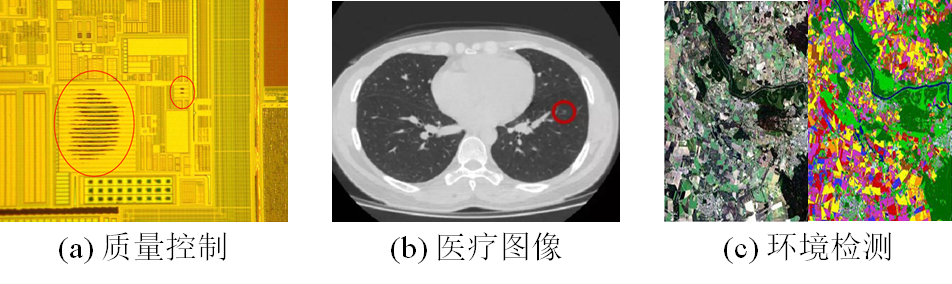
\includegraphics[width=1\linewidth]{figs/图像异常检测的应用.jpg}
	\caption{图像异常检测的具体应用}
	\label{fig:Specific application of image anomaly detection}
\end{figure}

图像异常检测属于视觉异常检测技术之一,是异常检测在图像领域的具体应用。图像异常检测专注于处理图像数据,旨在图像数据中识别出与正常模式或预期标准显著不同的区域或特征。目前,图像异常检测已广泛应用于各个领域。在质量控制方面,如\autoref{fig:Specific application of image anomaly detection}(a)所示,图像异常检测可以用于生产线上的产品检验,通过自动化检测产品外观,及时识别出缺陷或瑕疵,从而提高产品的合格率和客户满意度;在医学图像中,如\autoref{fig:Specific application of image anomaly detection}(b)所示,图像异常检测可帮助医生识别CT图像、核磁共振等影像中的病变区域;而在环境检测方面,如\autoref{fig:Specific application of image anomaly detection}(b)所示,图像异常检测可用于监测自然环境的变化,例如通过分析卫星图像来识别森林砍伐、污染或自然灾害的迹象。


\subsection{工业图像异常检测与定位}

工业图像异常检测旨在发现各类工业制品表面的各种可见性异常,比如布料、芯片、药物以及建筑材料的瑕疵。尽管这些异常可能极其微小,但在某些情况下会严重影响产品的正常功能,甚至带来安全隐患。这些异常可能出现在生产、运输或使用的任何环节,因此及时准确地检测这些问题对确保产品质量至关重要。工业图像异常检测不仅可以在生产过程中实现对产品质量的精确控制,还能提升生产效率、降低成本,从而促进全面的质量管理和生产优化。根据输出结果的粒度大小,工业图像异常检测任务可分为异常检测与异常定位两个子任务。

根据输出结果的粒度,工业图像异常检测任务可以细分为异常检测与异常定位。异常检测任务在图像级(image-wise)层面为每张图像生成整体的异常评分,用于对图像进行分类,即判断该图像是否包含异常;而异常定位任务则进一步在像素级(pixel-wise)层面为每个像素生成异常评分,从而实现异常区域的精确定位。例如,如\autoref{fig:Example of capsule}所示,对于一个胶囊图像,异常检测任务首先将其判定为“正常”或“异常”样本。如果判定为异常,还可以进一步识别异常的具体类型,如挤压、裂纹、破洞或刮蹭等。而异常定位任务则着眼于找出具体的异常区域,通常通过检测框或像素级别的分割图来标记异常的精确位置。

\begin{figure}[htb]
	\centering
	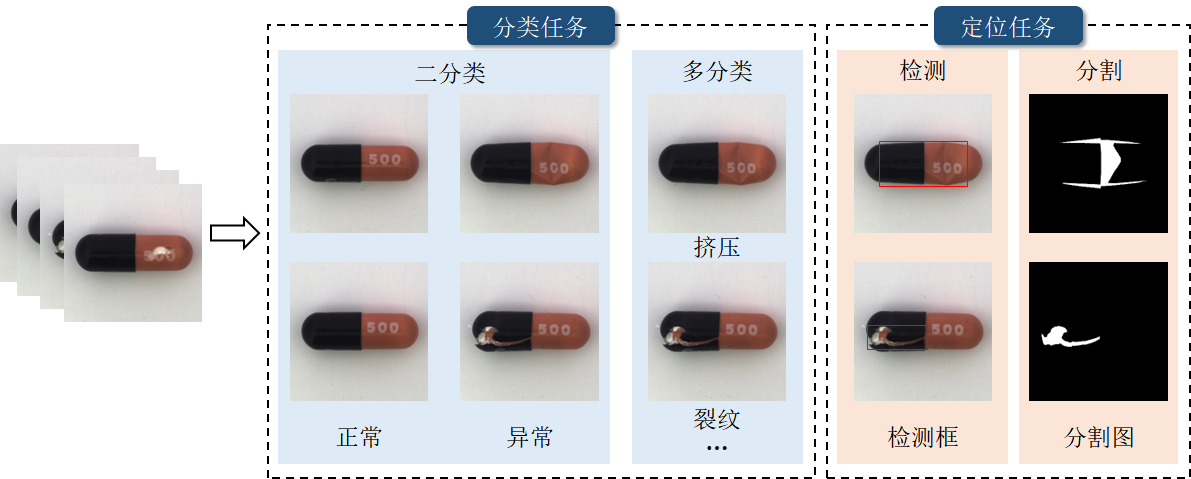
\includegraphics[width=1\linewidth]{figs/胶囊类别异常检测示例.png}
	\caption{胶囊类别图像异常检测}
	\label{fig:Example of capsule}
\end{figure}

与常规图像异常检测相比,工业图像异常检测与定位更侧重于像素级别的检测任务。在这一层面上,工业图像中的正常和异常模式之间的差异往往非常细微,加之背景复杂、异常区域的显著性较弱,使得检测任务具有更高的挑战性。像素级的检测不仅需要模型对图像细节有极高的敏感度,还必须能够有效应对不同类型的噪声与复杂的背景干扰,从而实现精准的异常定位。

\section{深度学习算法}

\subsection{自编码器}

自编码器(AutoEncoder, AE)是当前广泛使用的无监督学习方法之一,主要用于特征提取、数据压缩和维度降维。自编码器由两个主要部分组成:编码器(Encoder)和解码器(Decoder),通常采用对称的网络结构,如\autoref{fig:AE}所示。编码器的任务是将高维度的输入数据转换为低维度的隐含表示,从而实现数据压缩和降维;解码器则负责将这些低维度的抽象特征还原为与输入数据尽可能接近的输出,达到数据重构的目的。自编码器在多个领域都有广泛的应用,例如数据去噪、图像重构、数据降维、机器翻译以及异常检测等。特别是在异常检测中,自编码器通过学习正常数据的内在特征来构建模型,当输入的测试数据与正常数据有显著差异时,重构误差会较大,从而有效检测出异常。

与全连接神经网络类似,自编码器的节点之间也采用全连接方式。然而,不同于有监督学习方法,自编码器在无监督学习模式下进行训练,输入和输出都是无标签数据。通过对输入数据的深入学习,自编码器能够提取出数据的抽象特征,揭示数据的内在结构,为后续的任务提供更加简洁有效的特征表示。因此,自编码器的意义在于它能够自动学习数据的隐藏特征,减少维度和噪声的同时保留有价值的信息,极大地提升了模型在各类复杂任务中的性能和效率。

\begin{figure}[htb]
	\centering
	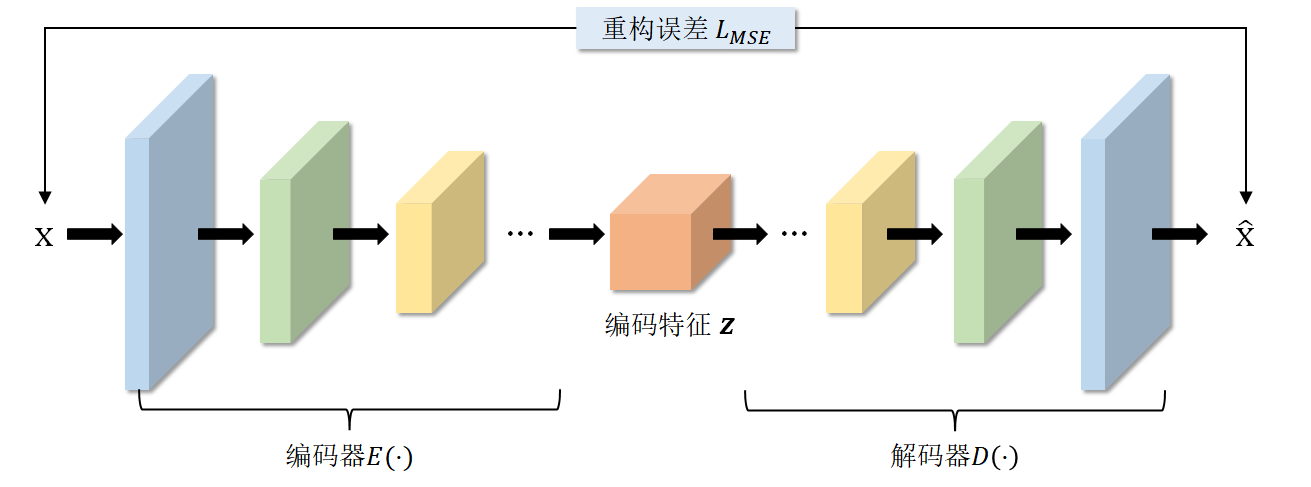
\includegraphics[width=0.9\linewidth]{figs/自编码器.png}
	\caption{自编码器}
	\label{fig:AE}
\end{figure}

整体上,自编码器的训练过程包括编码、解码和损失计算3个阶段。编码过程中,编码器$E(\cdot)$将高维输入样本$x$非线性映射地压缩到低维隐空间,并得到低维编码特征 $z$ ,其映射如\autoref{eq:encode}所示。

\begin{equation}
    \label{eq:encode}
    z = E(x).
\end{equation}

解码过程中,解码器对低维编码特征 $z$ 进行解码,通过函数 $D(\cdot)$ 对低维编码特征 $z$ 进行重构,并得到与输入样本 $x$ 尽量相似的重构样本 $\hat{x}$ ,其表达如\autoref{eq:decode}所示。

\begin{equation}
    \label{eq:decode}
    \hat{x}=D(z)=D(E(x)).
\end{equation}

最后,为了优化自编码器的性能,自编码器训练过程的最终目标是最小化输入样本 $x$ 与重构样本 $\hat{x}$ 之间的差异。常用均方误差(Mean-Square Error, MSE)作为损失函数进行自编码的训练,其表达如\autoref{eq:MSE} 所示。

\begin{equation}
    \label{eq:MSE}
    L_{MSE}=\frac{1}{N}\sum_{i=1}^{N}\vert\vert\hat{x}_i-x_i\vert\vert_2^2.
\end{equation}

其中,$N$ 是样本量,$\hat{x}_i$ 和 $x_i$ 分别代表第 $i$ 个重构样本和其对应的输入样本。最后采用反向传播算法\cite{lecun2012efficient}对网络参数进行调整,使重构误差最小化,以此达到获取输入样本特征的最佳抽象表示和数据压缩的目的。

\subsection{卷积神经网络}

卷积神经网络(Convolutional Neural Network,CNN)\cite{lecun1998gradient}是一种经典的前馈神经网络架构,广泛应用于计算机视觉领域,并在图像识别\cite{krizhevsky2012imagenet}、对象检测\cite{girshick2014rich}、情绪识别\cite{mollahosseini2017affectnet}等任务中取得了显著成功。当输入为图像时,CNN能够直接将图像作为网络的输入,避免了传统方法中繁琐的特征提取和数据重建步骤,从而实现了更加高效的端到端学习。CNN的优势在于其能够自动提取图像的多层次特征,包括颜色、形状、纹理以及更复杂的拓扑结构。通过卷积操作,它可以有效捕捉局部空间信息,并在不同的层级逐步抽象出图像的高阶特征。相比传统的全连接网络,CNN在处理二维图像时具有显著优势,因为其卷积核能够共享权重,极大地减少了参数数量,降低了模型的复杂度。此外,CNN具有良好的位移不变性、尺度不变性以及旋转不变性,能够较好地应对图像的平移、缩放和旋转等变化。在处理大型数据集和复杂任务时,CNN不仅在准确性上具有突出表现,还展现出较高的计算效率。正因为这些优势,CNN已成为图像识别\cite{krizhevsky2012imagenet}、目标检测\cite{ren2016faster}、语义分割\cite{long2015fully}、视频分析\cite{tran2015learning}等领域的主流模型之一。

\begin{figure}[htb]
	\centering
	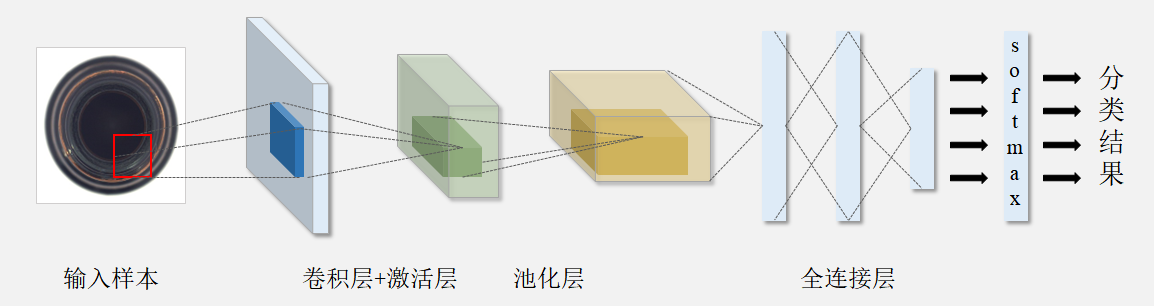
\includegraphics[width=1\linewidth]{figs/卷积神经网络结构.png}
	\caption{卷积神经网络结构}
	\label{fig:CNN Structure}
\end{figure}

\autoref{fig:CNN Structure}展示了卷积神经网络的经典结构,其一般是由卷积层、池化层、激活层、全连接层等堆叠构成的神经网络。下面依次介绍各组成模块:

\subsubsection{卷积层}

卷积层是CNN架构中的核心组成部分,主要用于局部特征的提取。它由一组卷积核组成,每个卷积核相当于一个特征提取器,用于识别输入数据中的模式,如边缘或纹理。卷积层的关键特点是权重共享,即同一组卷积核在输入数据上滑动,提取不同区域的特征。这样不仅大幅减少了参数量,还能更高效地处理图像信息。\autoref{fig:Conv Layer}展示了卷积层的工作过程:输入一个三维特征图,通过两个不同的卷积核进行卷积,提取出的特征图堆叠在一起,作为卷积层的输出。这种方式让CNN能从多个角度提取重要信息,同时保持较高的计算效率。

\begin{figure}[htb]
	\centering
	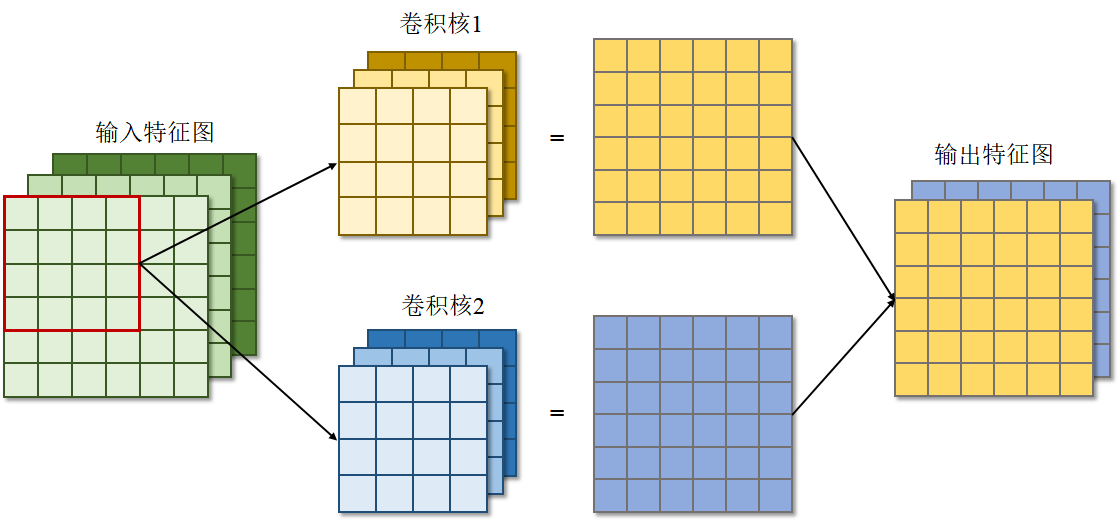
\includegraphics[width=0.7\linewidth]{figs/卷积层特征提取过程示例.png}
	\caption{卷积层特征提取过程示例}
	\label{fig:Conv Layer}
\end{figure}

\subsubsection{池化层}

池化层的主要功能是对特征图进行下采样,以减小尺寸,从而减少计算量、降低特征维度,并帮助防止过拟合。此外,池化层还能为网络引入一定的平移和旋转不变性。池化层通常在空间维度上操作,常见的类型包括最大池化(Max Pooling)、平均池化(Average Pooling)和全局平均池化(Global Average Pooling)。其中,最大池化提取池化窗口内的最大值,保留最显著的特征;平均池化计算池化窗口内的平均值;全局平均池化则是对整个特征图取平均,常用于分类任务的末端。\autoref{fig:Pooling Layer}展示了在池化窗口大小为$2\times2$、步幅为2的情况下,这三种池化操作的示例。池化操作通过减少特征图的分辨率,有效提高了模型的计算效率,同时保持了对图像关键特征的捕捉能力。

\begin{figure}[htb]
	\centering
	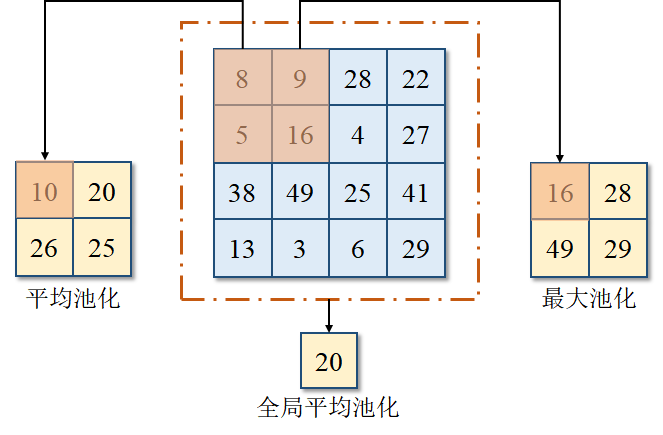
\includegraphics[width=0.7\linewidth]{figs/三种类型池化示例.png}
	\caption{三种类型池化示例}
	\label{fig:Pooling Layer}
\end{figure}

\subsubsection{激活层}

激活层也称为非线性层,在任何神经网络模型中都非常重要,它给网络模型引入了非线性,使得模型能够处理复杂的模式和数据。激活层通过激活函数实现,其主要作用是增强模型的表征能力和学习能力,使网络能够拟合和表达非线性关系。而激活函数通常具有以下几个特性:它是一个连续可导的非线性函数、设计简洁以避免增加计算复杂度,并且其输出值在合理的范围内。在CNN中,常用的激活函数主要有Sigmoid\cite{han1995influence}、Tanh\cite{lecun2012efficient}和ReLU\cite{simonyan2014very}等,它们的函数表达如\autoref{eq:activate functions}所示:

\begin{equation}
    \label{eq:activate functions}
    \begin{cases}
       sigmoid(x) = \frac{1}{1+e^{-x}} \\
       Tanh(x) = \frac{e^x - e^{-x}}{e^x + e^{-x}} \\
       ReLU = max(0,x)
    \end{cases}
\end{equation}

目前ReLU已成为了在CNN中最常用的激活函数,因为相比于其他激活函数,ReLU计算更简单高效。ReLU在 $x>0$ 时,导数值恒为1,这有效缓解了深度网络中的“梯度消失”问题,使得网络能够更快收敛。此外,ReLU的输出为0或 $x$ ,为模型引入了稀疏性,即很多神经元的激活值为0,从而提高了网络的计算效率。

\subsubsection{全连接层}

全连接层通常位于CNN结构的尾端,并常用于作为分类器。在全连接层中,每个神经元与前一层的所有神经元相连,因此该层包含了大量参数,往往占据了模型的大部分计算资源和存储空间。这种密集的连接方式在某些任务中具有很强的表达能力,但也容易导致过拟合和计算负担的增加。在现代的计算机视觉稠密预测任务(如图像分割、目标检测等)中,许多模型已逐步抛弃了全连接层,转而采用全卷积网络(Fully Convolutional Network, FCN)\cite{long2015fully}。全卷积网络通过用卷积层代替全连接层,保留了空间信息的完整性,且大幅减少了参数量,同时更适合处理像素级别的预测任务。

\subsection{残差网络}

随着数据量的增加,神经网络的深度也逐渐加深。然而,网络深度越深,在反向传播过程中容易出现梯度消失或梯度爆炸问题,导致模型难以有效训练和收敛。为了解决深层网络模型优化困难和性能下降的问题,残差网络(Residual Network, ResNet)\cite{he2016deep}采用残差连接的形式,将模块的输入直接与模块输出直接相加,并对其激活。这种设计有效缓解了梯度消失问题,使得深度网络更易于训练。残差模块的基本结构如\autoref{fig:Residual Block}所示,其中 $x$ 为输入,$F(x)$  为残差函数。残差网络的目标是通过拟合残差 $H(x)-x$ ,而不是直接拟合原始映射 $H(x)$,这样 $x$ 可以通过简单的恒等映射直接与 $F(x)$  相加,然后经过非线性层激活得到输出。残差块中这种连接方式称为“快捷连接”,这种方式允许原始输入和处理后的特征共同传递到下一层,不仅避免了模型过拟合问题,还能够有效防止梯度消失现象。

\begin{figure}[htb]
	\centering
	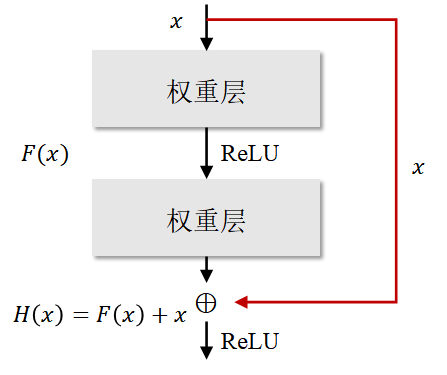
\includegraphics[width=0.5\linewidth]{figs/残差模块.png}
	\caption{残差模块示例}
	\label{fig:Residual Block}
\end{figure}

不同的ResNet模型如\autoref{fig:ResNets}所示,它们根据网络的层数命名,例如ResNet-18就表示该模型是具有18层网络层的 ResNet 模型。可以看到,在ResNet的结构中,第一阶段通常包含一个步幅为2的“$7\times7$ 卷积+ $3\times3$ 最大池化”操作,这部分通常被称为网络的茎结构(stem),负责输入图像的初步处理。接下来的网络由四个层级(layer)组成,每个层级都由多个相同的残差模块堆叠而成。这些模块在相同的分辨率下进行操作,并提取不同层次的特征。当进入下一个层级时,ResNet会对特征图进行尺度下采样,同时通过增加卷积核的数量进行通道扩展。这种设计使得不同层级输出的特征图具有不同的分辨率,构成了输入图像的多层次特征表示。这种逐层下采样和通道扩展的方式,使ResNet能够在保留更多细节信息的同时,逐渐提取出更抽象的高级特征,从而提升模型的识别和分类能力。

\begin{figure}[htb]
	\centering
	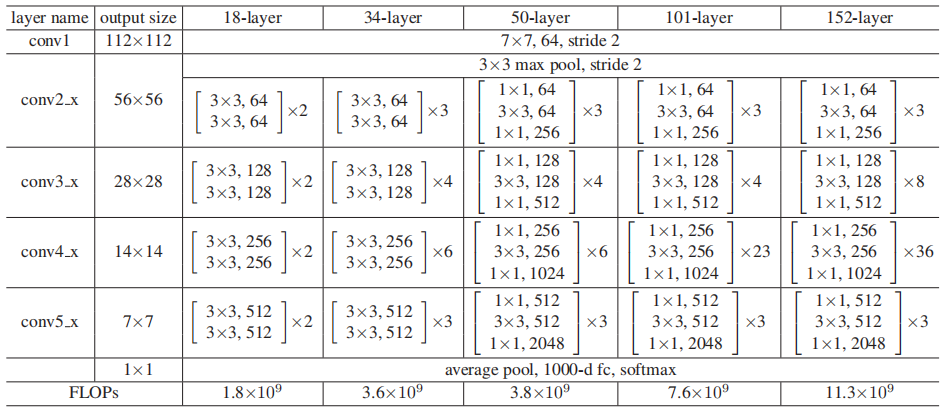
\includegraphics[width=1\linewidth]{figs/不同ResNet模型结构.png}
	\caption{不同ResNet模型结构}
	\label{fig:ResNets}
\end{figure}

ResNet在拟合复杂的分类函数方面表现卓越,能够显著提高分类的准确率,同时加速深度神经网络的训练。由于其出色的性能,ResNet已在多个领域得到了广泛应用,包括图像识别、时间序列预测、图像超分辨率、行人检测与重建等任务。作为目前计算机视觉领域中最常用的骨干网络,ResNet在复杂场景的视觉任务中表现出了高度的准确性和泛化能力。

\subsection{注意力机制}

人类对世界的观察和信息获取通常是选择性的。在认知科学中,由于信息处理的瓶颈,人类在某一时刻只能关注一部分信息,而忽略其他可见的信息。同样地,在深度神经网络处理图像数据时,也不应对整张图像逐一进行信息提取与识别,而是需要聚焦于物体所在的关键区域,再进行相关的信息提取与识别。基于这一理念,注意力机制(Attention Mechanism)\cite{woo2018cbam}在深度学习中应运而生。注意力机制源于对人类视觉系统的研究,它通过模拟人类选择性关注的重要区域,提高了模型的有效性。作为一种即插即用的技术,注意力机制显著增强了神经网络处理信息的能力,已成为神经网络结构中的常见组件,广泛应用于图像字幕生成、动作识别、语音识别等任务中。注意力机制能够帮助网络自动选择最具信息量的特征,减少不相关信息的干扰,进而提升模型的性能和效率。

\begin{figure}[htb]
	\centering
	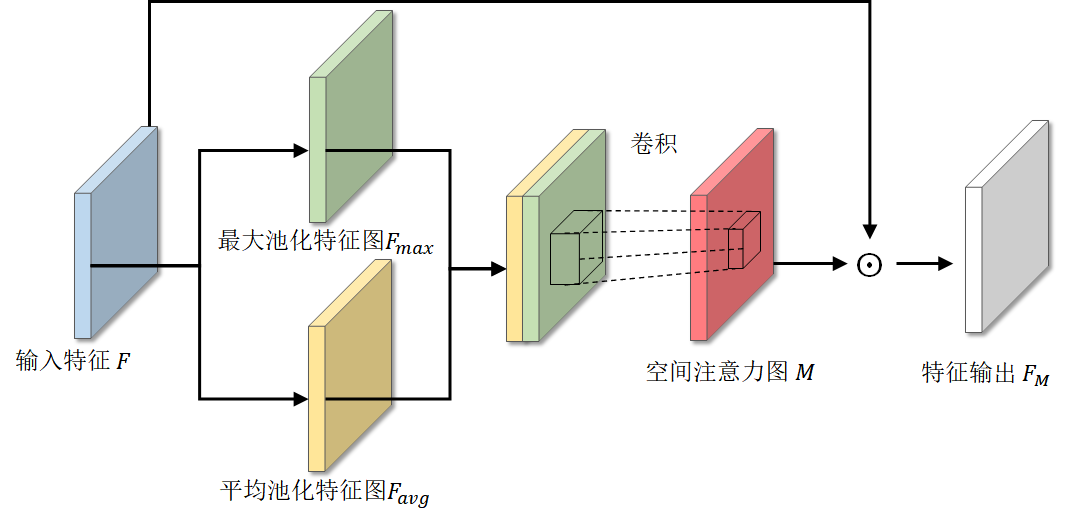
\includegraphics[width=0.8\linewidth]{figs/空间注意力机制.png}
	\caption{空间注意力机制}
	\label{fig:Attention Mechanism}
\end{figure}

\autoref{fig:Attention Mechanism}介绍了本文算法所采用的空间注意力机制,首先对输入特征 F 同时进行最大池化和平均池化操作,分别得到最大池化特征图 $F_{max}$  和平均池化特征图 $F_{avg}$,池化过程表示如\autoref{eq:Pool}所示:

\begin{equation}
    \label{eq:Pool}
    F_{max} = MaxPool(F), F_{avg}=AvgPool(F).
\end{equation}

其次,将这两个特征图进行卷积操作和非线性映射,得到特征映射 $M$,该过程表示为\autoref{eq:Feature Mapping}:

\begin{equation}
    \label{eq:Feature Mapping}
    M = \sigma(Conv([F_{max},F_{avg}])),
\end{equation}
\noindent
其中 $\sigma(\cdot)$ 表示激活函数,如ReLU激活函数,$Conv(\cdot)$ 表示卷积操作,$[\cdot,\cdot]$ 表示特征图拼接。卷积处理后得到的 $M$ 即是空间注意力图,其表示每个空间位置的重要性权重。此时,可以对原始特征 $F$ 进行加权计算,得到加权后的输出特征图 $F_M$,其表示如\autoref{eq:F_M}所示:

\begin{equation}
    \label{eq:F_M}
    F_M = M \bigodot F,
\end{equation}
\noindent
其中 $\bigodot$ 表示逐元素相乘,也称为Hadamard乘积。

空间注意力机制除了能够保留了特征空间位置的关键信息,同时能够聚焦于对当前任务更为关键的信息,弱化无用的特征信息,特别是在处理异常检测等任务时,空间注意力机制能够有效处理与异常检测任务的背景噪声,提高异常检测的性能。

\section{数据集与评价指标}

\subsection{数据集介绍}

为了衡量本文所提出算法的有效性,本文选用了目前图像异常检测领域使用最广泛的工业图像异常检测数据集MVTec AD(MVTec Anomaly Detection)作为实验的基准数据集。

MVTec AD\cite{bergmann2019mvtec} 是 MVTec 公司于2019年针对工业图像缺陷检测所发布的一个基准测试数据集。与之前的异常检测数据集不同,该数据集模仿了工业实际生产场景,并且主要用于无监督异常检测。数据集为异常区域都提供了像素级标注,是一个全面的、包含多种物体、多种异常类型的数据集。该数据集一共有5354张高清图像,图像的分辨率从 $700\times700$ 到 $1024\times1024$ 不等,其中3629张用于训练,1725张用于测试。训练集中只包含无缺陷的正常图像,而测试集包括了正常图像以及不同缺陷类型的异常图像,测试集的真实标签即包括了用于图像级异常检测的标签,还包括了用于像素级异常定位的掩码。此外,MVTec AD中图像的异常类型也非常多样,包括例如裂纹、污垢、划痕以及各种结构缺失等70多种不同类型,并且这些异常是自然产生的,目的是产生与实际生产中相符的异常图像,更加贴近实际的工业检验场景,非常适合用于图像异常检测算法的性能的评估。

MVTec AD一共涵盖了15种不同类别的数据,其中5种纹理类数据均为不同纹理结构的图像,比如包含规律性纹理的地毯(carpet),或者无规律纹理的瓷砖等,还有10种结构物体类数据,这类数据既包含了特定外观、刚性变化的物体,如瓶口(bottle),也有可形变的物体,如电缆(cable),或者自然物体,如榛子(hazelnut)等。\autoref{fig:MVTec AD}展示了MVTec AD全部类别的图像示例,第一行为正常图像,第二行和第三行分别为异常图像与对应的真实掩码标签。

\begin{figure}[H]
	\centering
	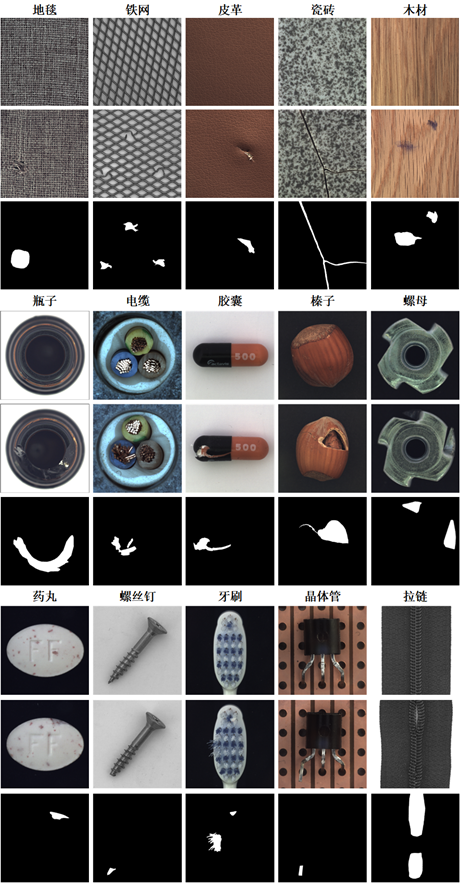
\includegraphics[width=0.77\linewidth]{figs/MVTecAD.png}
	\caption{MVTec AD数据集中的正常图像、异常图像以及对应的真实掩码标签}
	\label{fig:MVTec AD}
\end{figure}

\subsection{评价指标介绍}

遵循现有工作的惯例,本文采用采用受试者工作特性曲线下面积(Area Under Receiver Operating Characteristic curve, AUROC)和区域重叠分数(Per-Region Overlap score, PRO)来评估本文算法的性能。PRO分数是AUROC指标的补充,由Bergmann等人\cite{bergmann2020uninformed}提出,由于AUROC在像素级异常检测任务中,易偏向较大面积的异常区域,对异常检测性能的评估缺乏公正性,因此提出了PRO分数。

\subsubsection{图像级AUROC和像素级AUROC}

AUROC可分为图像级与像素级。图像级AUROC(Image-wise AUROC, I-AUPOC)指标是针对图像级异常检测任务的受试者工作特性曲线下面积,而像素级 AUROC(Pixel-wise AUROC, P-AUROC)指标是针对像素级异常定位任务的像素级的受试者工作特性曲线下面积。两个指标都需要计算AUROC,只不过前一个是从图像角度出发,即针对图像级异常得分进行评估,后一个是从像素角度出发,即针对像素级异常得分图进行评估。

AUROC指的是受试者工作特性(Receiver Operating Characteristic curve, ROC)曲线下的归一化面积,是一个衡量分类模型性能在多阈值设定下的重要的评价指标,通常用于二分类任务(0/1 两个类),具有对类别不平衡不敏感、不随正负样本比例变化而明显变化等优点。AUROC度量了在当前模型对数据的可分离性,综合反映了模型区分类别的能力,其值越高表示模型有更大的把握区分好 0/1 类别。一个优秀的模型AUROC值接近1,这意味着它对数据具有良好的可分离性,如果 AUROC等于1,则说明在某个阈值下,0/1 两类数据能够被完全区分开,而当AUROC为0.5时,这意味着模型没有任何分离能力\cite{narkhede2018understanding}。

\begin{figure}[H]
	\centering
	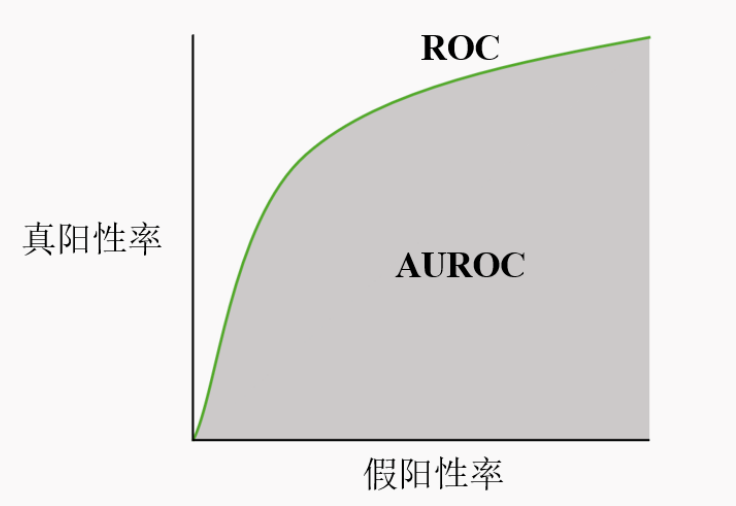
\includegraphics[width=0.5\linewidth]{figs/ROC.png}
	\caption{ROC曲线示例}
	\label{fig:ROC}
\end{figure}

\autoref{fig:ROC}展示了一个ROC曲线的示例,该曲线展示了分类模型在不同阈值设定下的性能。ROC曲线的横轴为假阳性率(False Positive Rate, FPR),纵轴为真阳性率(True Positive Rate, TPR)。通过在不同阈值下计算FPR和TPR,得到对应坐标系中的多个点,将这些点连成曲线即可形成ROC曲线(如\autoref{fig:ROC}中的绿色曲线)。ROC曲线下的面积即为AUROC,代表模型的分类性能。\autoref{fig:ROC}的灰色阴影区域就是AUROC的面积,面积越大,表示模型的区分能力越强。而 FPR 和 TPR 的计算公式如\autoref{eq:FPR&TPR}所示:

\begin{equation}
    \label{eq:FPR&TPR}
    FPR = \frac{FP}{TN + FP}, TPR = \frac{TP}{TP + FN},
\end{equation}

其中 FP(False Positive)表示被模型错误判断为正类的负样本数,TP(Ture Positive)表示被模型正确判断为正类的正样本数,FN(False Negative)表示被模型错误判断为负类的正样本数,TN(True Negative)表示被模型正确判断为负类的负样本数。

\subsubsection{PRO分数}

PRO分数\cite{bergmann2020uninformed}是为了减少像素级异常检测指标评估时存在的尺度偏好而提出的,用于评估模型在图像分割任务中对局部区域(区域级)的准确度,并在评估指标时对不同尺度的异常区域都赋予了相同的权重。特别是在异常检测与定位任务中,PRO用于衡量模型在预测异常区域时,与真实异常区域的重叠程度。具体来说,PRO分数表示了不同区域重叠曲线下的归一化面积,通过计算预测区域与真实区域的重叠比例,逐步调整阈值,生成一条曲线,用来反映模型的区域定位性能。它反映了模型对不同尺度异常区域的整体检测效果,值越大表示模型定位不同尺度异常的能力越强。

\begin{figure}[H]
	\centering
	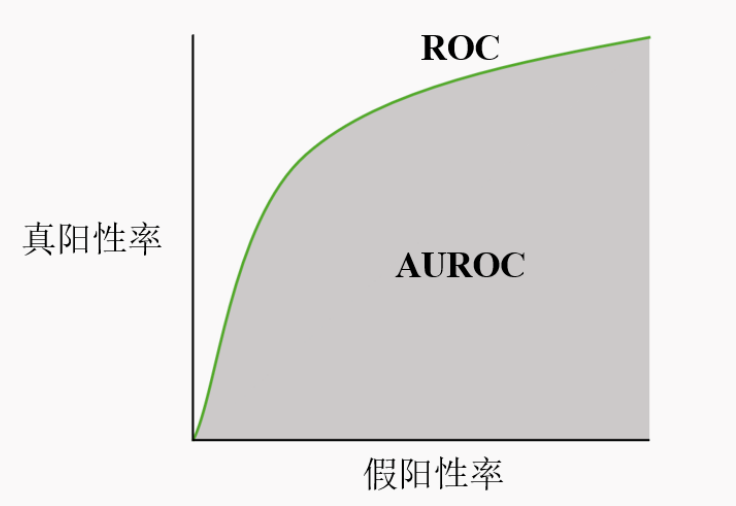
\includegraphics[width=0.5\linewidth]{figs/PRO.png}
	\caption{PRO曲线示例}
	\label{fig:PRO}
\end{figure}

与ROC曲线关注整个图像的分类不同,PRO曲线更注重局部区域的匹配程度。PRO曲线下的面积可以用来评价模型的局部区域检测效果,值越大表示模型在区域级别上的定位越准确。如\autoref{fig:PRO}所示,为了计算PRO分数,同样需要选取阈值得到像素的二值识别结果,根据真实掩码和模型预测结果计算每个真实缺陷区域的像素级 FPR 和平均覆盖率(PRO),其中PRO值即为真实异常区域和预测区域的重叠百分比。再以FPR为横轴,PRO值作为纵轴绘制不同阈值设定下的曲线(称为PRO曲线),最后计算曲线下的归一化面积作为PRO分数。

\section{本章小结}

章首先介绍了异常检测和工业图像异常检测与定位的相关定义。其次,对异常检测领域的常用的深度学习算法框架:自编码器、卷积神经网络、残差网络、注意力机制进行了介绍。最后,本章介绍了本文所使用的基准数据集以及图像异常检测领域三个常用的性能评价指标。

\chapter{说明}
\subsection{这是小标题}
emmmmm
\subsubsection{这是小小标题}
搞这么多层大丈夫?

\section{公式}
简单行内公式 $a+b=233$,超高公式会被压缩 $\frac{1}{2}=0.5$ 或者使用
\lstinline`\displaystyle` 防止被压缩:$\displaystyle \frac{1}{2}=0.5$。

简单的不标号单行公式
$$a_0+a_1+a_2=\sqrt{233}$$
需要标号和起名的公式如\autoref{eq:eqtest} 所示。测试下 autoref \autoref{eq:eqtest}
\begin{equation}
    \label{eq:eqtest}
    a_0 + a_1 + a_2 = \sqrt{233}
\end{equation}

\section{特殊符号}

用\href{http://detexify.kirelabs.org/classify.html}{
    http://detexify.kirelabs.org/classify.html}画出来。

\section{参考文献的引用}

\LaTeX{} 中要求参考文献使用 \lstinline`\cite` 进行参考引用,若论文要求中说明需在
文字的右上角注明引用,请使用命令 \lstinline`\cite` 进行参考引用。举个不恰当的例
子,比如本论文模板的原版“LaTeX-Template-For-NPU-Thesis”\cite{NWPUThesisLaTeXTemplate}
要求务必声明引用,同时预配置了插件“math-symbols”\cite{MathSymbolsinLaTeXbypolossk}。
对组件的引用是每一名科学工作者的基本素养(一本正经)。对于需要引用但是并不需要明
确指明引用位置的文献,请使用 \lstinline`\nocite` 命令。

在此同时感谢真正的 dalao 高德纳开发了全世界版本号最接近 $\pi$ 的软件
\LaTeX \cite{knuth1986the}\nocite{lamport1989latex}。

测试引用文献 \cite{szegedy2015going, shen2021peridynamic, chen2014maiyuan, chen2018autonomous}。
其中倒数第二篇为中文文献,最后一篇为会议文献。

\section{标点符号的选择}

根据《中华人民共和国国家标准 GB/T 15834-1995》及《出版工作中的语言文字规范》中提
及,“科学技术中文图书,如果涉及公式、算式较多,句号可以统一用英文句号‘.’,省略
号用英文三个点的省略号‘…’”。如果您是中文的科技论文写作者,建议您使用全角英文句
号“\lstinline`.`”间隔句子。如果是人文学科则可以不做处理。您也可以在一开始先使用
中文句号‘。’,最后批量替换即可。

\section{萌新如何编译}

\begin{enumerate}
    \setlength{\itemsep}{0pt}
    \item 安装正确版本的 TexLive 2021
    \item 使用自带的 TeXworks 打开 \lstinline`yanputhesis-sample.tex`
    \item 左上角下拉框选择工具
    \item 依次使用 \lstinline`XeLaTeX-BibTeX-XeLaTeX-XeLaTeX` 编译
\end{enumerate}

\section{如何生成盲评版本}

\begin{enumerate}
    \setlength{\itemsep}{0pt}
    \item 在这份样例当中,已经将标题页可能用到的作者姓名、导师姓名添加了空白盲评
          标记 \lstinline`\blindreview{text}`。如果需要生成盲评版本,则需要将文档类型
          设置为 \lstinline`blindreview=true`,这样便可得到标题页不含作者与导师姓名的
          版本。
    \item 在致谢中,除了导师名字之外,其他老师、同学的名字也应当隐去。同样可以将
          姓名添加空白盲评标记 \lstinline`\blindreview{text}` 来得到留空版本的结果。
    \item 一般正文中不建议出现留空,因此推荐另外两种盲评标记,涂黑或者打星。使用
          \lstinline`\blackbox{text}` 命令将姓名添加涂黑盲评标记,文本会替换为与文字相
          同长度的黑色方块,制造涂黑效果。或者使用 \lstinline`\markname{text}` 命令将
          姓名添加打星盲评标记,姓名将替换成 3 个星号“***”。
    \item 下面给出示例(通过开启盲评选项查看效果):
          \begin{enumerate}
              \setlength{\itemsep}{0pt}
              \item 不添加任何盲评标记:“感谢某某某教授的悉心指导。”
              \item 使用了空白盲评标记:“感谢\blindreview{某某某}教授的悉心指导。”
              \item 使用了涂黑盲评标记:“感谢\blackbox{某某某}教授的悉心指导。”
              \item 使用了打星盲评标记:“感谢\markname{某某某}教授的悉心指导。”
          \end{enumerate}
\end{enumerate}

\section{如何生成学位论文评阅人和答辩委员会名单}

\begin{enumerate}
    \setlength{\itemsep}{0pt}
    \item 在这份样例当中,已经预设置了盲评学位论文评阅人和答辩委员会名单,实现代码可
          参考\autoref{code:makeBlindReviewerCommitteePage} 所示,明审版本可参考
          \autoref{code:makeOpenReviewerCommitteePage} 所示。
    \item 在学位论文评阅人名单中分为两种情况,即盲评与明审。请根据自身情况填写评
          委信息。如果是盲评,使用命令 \lstinline`\fullBlindReview{num}` 来生成
          盲评表格,其中参数 \lstinline`num` 表示盲评专家人数,一般是 3 或 5 人。
          如果是明审,使用命令 \lstinline`\expert{name}{title}{university}`
          登记评委信息,其中参数 \lstinline`name`、\lstinline`title`、
          \lstinline`university` 分别为专家的姓名、职称、学校。
    \item 答辩委员会需登记四个信息:答辩时间、答辩主席、答辩评委以及答辩秘书。其
          中,答辩时间为 \lstinline`\committee` 命令后的第一个参数,其余分别使用
          \lstinline`\defenseChair`、\lstinline`\committeeMember`、
          \lstinline`\defenseSecretary` 命令登记专家个人信息,用法与
          \lstinline`\expert` 命令一致。
\end{enumerate}

\begin{lstlisting}[language={TeX}, label={code:makeBlindReviewerCommitteePage},
    caption={盲评样例 makeBlindReviewerCommitteePage.tex}]
\makeCommitteePage{
    \reviewers{\fullBlindReview{5}}
    \committee{2023 年 x 月 y 日}{
        \defenseChair{赵钱孙}{教授}{西北工业大学}
        \committeeMember{周吴郑}{教授}{西北工业大学}
        \committeeMember{冯陈褚}{教授}{西北工业大学}
        \committeeMember{蒋沈韩}{教授}{西北工业大学}
        \committeeMember{朱秦尤}{教授}{西北工业大学}
        \committeeMember{何吕施}{教授}{西北工业大学}
        \committeeMember{孔曹严}{教授}{西北工业大学}
        \defenseSecretary{金魏陶}{教授}{西北工业大学}
    }
}
\end{lstlisting}

\begin{lstlisting}[language={TeX}, label={code:makeOpenReviewerCommitteePage},
    caption={明审样例 makeOpenReviewerCommitteePage.tex}]
\makeCommitteePage{
    \reviewers{
        \expert{周吴郑}{教授}{西北工业大学}
        \expert{冯陈褚}{教授}{西北工业大学}
        \expert{蒋沈韩}{教授}{西北工业大学}
        \expert{朱秦尤}{教授}{西北工业大学}
        \expert{何吕施}{教授}{西北工业大学}
    }
    \committee{2023 年 x 月 y 日}{
        \defenseChair{赵钱孙}{教授}{西北工业大学}
        \committeeMember{周吴郑}{教授}{西北工业大学}
        \committeeMember{冯陈褚}{教授}{西北工业大学}
        \committeeMember{蒋沈韩}{教授}{西北工业大学}
        \committeeMember{朱秦尤}{教授}{西北工业大学}
        \committeeMember{何吕施}{教授}{西北工业大学}
        \committeeMember{孔曹严}{教授}{西北工业大学}
        \defenseSecretary{金魏陶}{教授}{西北工业大学}
    }
}
\end{lstlisting}

\cleardoublepage

\chapter{插入图表以及如何引用}
\chaptermark{插入图表以及如何引用}

\section{表格}

使用 \href{http://www.tablesgenerator.com/}{http://www.tablesgenerator.com/} 生
成,可粘贴Excel。效果如表\ref{my-label}所示。注意表中的字号(五号)和表格宽度(
通栏)。外部请用 \lstinline`table` 环境,内部使用 \lstinline`tabularx` 即可。

\begin{table}[!h]
    \centering
    \caption{表格标题}
    \label{my-label}
    \begin{tabularx}{\textwidth}{CCCC}
        \toprule
        $A$ & $B$ & $A+B$ & $A\times B$ \\ \midrule
        1   & 6   & 7     & 6           \\
        2   & 7   & 9     & 14          \\
        3   & 8   & 11    & 24          \\
        4   & 9   & 13    & 36          \\
        5   & 10  & 15    & 50          \\ \bottomrule
    \end{tabularx}
\end{table}

\begin{table}[!h]
    \centering
    \caption{指定宽度与对齐方式}
    \label{my-label-2}
    \begin{tabularx}{\textwidth}{|P{2cm}|O{3cm}|Q{4cm}|C}
        \toprule
        \SI{2}{\centi\metre} & \SI{3}{\centi\metre} & \SI{4}{\centi\metre} & Other \\ \midrule
        1                    & 6                    & 7                    & 1     \\
        2                    & 7                    & 9                    & 2     \\
        3                    & 8                    & 11                   & 3     \\ \bottomrule
    \end{tabularx}
\end{table}

\section{插图}

请直接使用 \lstinline`figure` 环境,内部使用 \lstinline`includegraphics` 即可。
如果需要多张子图排版,请在 \lstinline`figure` 环境内部使用 \lstinline`minipage`
预先设置总的浮动体宽度,然后再使用 \lstinline`subfigure` 环境进行排版。

测试下文章内的图片引用。如\autoref{fig:example} 和\autoref{fig:example2} 所示,
这是两幅插图。在这其中\autoref{subfig:example2-subfig1} 是第一幅子图,
\autoref{subfig:example2-subfig2} 是第二幅子图。

\begin{figure}[htb]
    \centering
    
\includegraphics[scale=0.2]{poster.png}
    \caption{
        这里是个普通的标题
    }
    \label{fig:example}
\end{figure}

\begin{figure}[htb]
    \centering
    \begin{minipage}[t]{0.96\textwidth}
        \centering
        \begin{subfigure}[t]{0.47\textwidth}
            \centering
            
\includegraphics[scale=0.1]{poster.png}
            \caption{\label{subfig:example2-subfig1}}
        \end{subfigure}
        \begin{subfigure}[t]{0.47\textwidth}
            \centering
            
\includegraphics[scale=0.1]{poster.png}
            \caption{\label{subfig:example2-subfig2}}
        \end{subfigure}
    \end{minipage}
    \caption{这里是另一个普通的标题}
    \label{fig:example2}
\end{figure}


\begin{figure}
	\centering
	\includegraphics[width=0.7\linewidth]{../../图/本文工作}
	\caption{}
	\label{fig:}
\end{figure}
\section{插入源代码}

这里给出一个 Hello World 的样例,如\autoref{code:hello-world} 所示。

\begin{lstlisting}[language={C++}, label={code:hello-world},
    caption={Hello World.cpp}]
#include <iostream>
using namespace std;

int main()
{
    // output "Hello World!"
    cout << "Hello World!" << endl;
    return 0;
}
\end{lstlisting}

\section{引用以及其他编写建议}

\LaTeX 提供了 \lstinline`ref` 和 \lstinline`autoref` 两种引用方式,其中前者只显
示序号,后者可以显示提示语,如“\autoref{code:hello-world}”表示引用代码,
而“\autoref{subfig:example2-subfig2}”表示引用图片的子图.为了方便引用以及作者阅读,
本人强烈建议使用 \lstinline`autoref` 来统一处理引用问题,同时在每一个
\lstinline`autoref` 添加提示语,如 \lstinline`fig` 和 \lstinline`tab` 分别表示插
图和表格。

由于 \XeLaTeX 在处理中文时,会自动在中文之间添加空格,所以请放心地在编写文档时换
行,防止某一行过长导致阅读时的不便。另外中英文之间的空格(包括命令)并未做严格限
制。本文推荐除在不影响最终成文的结果这一前提下,为保持文档的美观与易读,请自行选
择合适的编写方式。

\cleardoublepage
%%=============================================================================%
%% 参考文献以及附录
%%-----------------------------------------------------------------------------%
%% \bibliographystyle{nputhesis}                               % GB/T 7714-2015 格式
\bibliographystyle{nputhesis-noslash}                       % 参考文献改进格式
\bibliography{reference}                                    % 参考文献
\appendix
\chapter{一份说明 顺便测试英文标题 Title}

强烈不推荐英文标题!仅供测试,擅自使用后果自负。

\section{测试附录子标题}

这是一份附录,请放置一些独立的证明、源代码、或其他辅助资料。

\nomenclature{$r$}{圆(或球)的半径}
\nomenclature{$C$}{圆的周长}
\nomenclature{$S$}{圆的面积}

\begin{equation}
    C = 2 \pi r
\end{equation}

\begin{equation}
    S = \pi r^2
\end{equation}

\cleardoublepage

\chapter{另一份说明}

这是另一份附录,请放置一些独立的证明、源代码、或其他辅助资料。

\nomenclature{$S_{\text{sphere}}$}{球的表面积}
\nomenclature{$V_{\text{sphere}}$}{球的体积}

\begin{equation}
    S_{\text{sphere}} = 4 \pi r^2
\end{equation}

\begin{equation}
    V_{\text{sphere}} = \frac43 \pi r^3
\end{equation}

\cleardoublepage
%%=============================================================================%
%% 文档附页部分(致谢、参加科研情况、知识产权与原创性声明)
%%-----------------------------------------------------------------------------%
\backmatter                                                 % 文档附页部分
%%-----------------------------------------------------------------------------%
\begin{acknowledgements}                                    % 致谢开始
    感谢我的老师和我的朋友们……
\end{acknowledgements}                                      % 致谢结束
%%-----------------------------------------------------------------------------%
\begin{accomplishments}                                     % 参加科研情况开始
    [1] ...
\end{accomplishments}                                       % 参加科研情况结束
%%-----------------------------------------------------------------------------%
\makestatement                                              % 知识产权与原创性声明
%%=============================================================================%
%% 文档结束
%%-----------------------------------------------------------------------------%
\end{document}
%%=============================================================================%


%% 
%% This work consists of the file  yanputhesis.dtx
%% and the derived files           yanputhesis.ins,
%%                                 yanputhesis.pdf,
%%                                 yanputhesis.cls.
%% 
%%
%% End of file `yanputhesis-sample.tex'.
